\documentclass{article}

% Language setting
% Replace `english' with e.g. `spanish' to change the document language
\usepackage[polish]{babel}

% Set page size and margins
% Replace `letterpaper' with `a4paper' for UK/EU standard size
\usepackage[a4paper,top=2cm,bottom=2cm,left=3cm,right=3cm,marginparwidth=1.75cm]{geometry}

% Useful packages
\usepackage{polski}
\usepackage[utf8]{inputenc}
\usepackage{amsmath}
\usepackage{graphicx}
\usepackage[colorlinks=true, allcolors=blue,unicode]{hyperref}
\usepackage{courier}
\usepackage[T1]{fontenc}
\usepackage{lastpage}

\usepackage{fancyhdr}
\pagestyle{fancy}
\fancyhead[L]{Specyfikacja implementacyjna}
\fancyhead[C]{}
\fancyhead[R]{Kamil Fryszkowski, Oskar Biwejnis}
\cfoot{\thepage/\pageref{LastPage}}


\title{Specyfikacja implementacyjna projektu w języku C}
\author{Kamil Fryszkowski, Oskar Biwejnis}

\begin{document}


\maketitle
\thispagestyle{fancy}
\section{Wstęp}
Celem projektu jest stworzenie programu w języku C, który będzie w stanie znajdować najkrótszą ścieżkę w pomiędzy dwoma wierzchołkami w danym grafie ważonym skierowanym. Użyte zostaną do tego algorytmy BFS oraz Dijkstry. Środowiskiem programistycznym będzie Linux, kod będzie pisany przy użyciu Vim, a wykorzystanym sposobem współpracy i wersjonowania - GIT.
Używane biblioteki języka C:
\begin{itemize}
\item \texttt{\footnotesize stdio.h} - odpowiedzialna za podstawowe komendy wejścia i wyjścia


\item \texttt{\footnotesize stdlib.h} - odpowiedzialna za komendy takie jak \texttt{\footnotesize rand, malloc} i inne


\item \texttt{\footnotesize time.h} - odpowiedzialna za pobranie ziarna do generatora liczb losowych
\end{itemize}

\section{Struktury danych}
Do poprawnego funkcjonowania programu niezbędne będzie zaimplementowanie następujących struktur danych:\\
\begin{enumerate}
\item Do przechowywania grafu użyta zostanie lista sąsiedztwa \texttt{graph\_t}, która będzie dwuwymiarową tablicą par liczb \texttt{\footnotesize <wierzcholek>, <waga>}. Informacją o tym, z którego wierzchołka wychodzi dane połączenie będzie indeks X tablicy. Wymiar X tablicy będzie zdefiniowany poprzez ilość wierzchołków równą wiersze * kolumny. Wymiar Y tablicy będzie równy 4, ponieważ taka jest maksymalna liczba krawędzi w grafie przypominającym kartkę w kratkę. Niewykorzystane pola będą zawierały wartość \texttt{\footnotesize null}.\\
Tekstowa reprezentacja przechowywania grafu:\\\\
\begin{tabular}{ccccc}
\textbf{X\textbackslash{}Y} & \textbf{0} & \textbf{1} & \textbf{2} & \textbf{3} \\
\textbf{0}                  & 1, 0.5..          & 4, 0.7..         & null       & null       \\
\textbf{1}                  & 2, 0.5..     &  5, 0.6...     & null       & null       \\
\textbf{2}                  & 3, 0.3..          & 1, 0.1..          & 6, 0.4..         & null      \\
\end{tabular}
\item Kolejka FIFO użyta zostanie przy działaniu algorytmu BFS. W kolejce tej, pierwszy wprowadzony element będzie pierwszym wyjętym. Do jej implementacji wykorzystana zostanie tablica statyczna, ponieważ znana jest jej długość - równa liczbie wierzchołków. Utworzone będą dwa wskaźniki p i k,  wskazujące kolejno początek i koniec kolejki. Przy dokładaniu elementów inkrementowany będzie wskaźnik k, a przy wyjmowaniu wskaźnik p. Możliwe operacje na kolejce:

\item Kolejka priorytetowa niezbędna będzie do poprawenego działania algorytmu Dijkstry. Priorytem według które będą wyjmowane elementy z kolejki będzie wartość \texttt{d[v]}, mówiąca o długości najkrótszej ścieżki do danego wierzchołka z wierzchołka startowego w danym momencie działania algorytmu. W celu szybszego wyjmowania elementów z kolejki, zostanie ona zaimplementowana na strukturze kopca.
\end{enumerate}
\section{Tryby pracy programu}
\begin{enumerate}
    \item Tryb \texttt{loadMode} służy do pracy z gotowym plikiem, na podstawie którego zostanie utworzony graf oraz ruchomiony zostanie algorytm Dijkstry w celu znalezienia najkrótszej ścieżki.
    \item Tryb \texttt{allRandMode} wygeneruje graf z losowymi krawędziami pomiędzy wierzchołkami oraz losowymi wagami, następnie znajdzie najkrótszą ścieżkę algorytmem Dijkstry.
    \item Tryb \texttt{conMode} wygeneruje graf podobnie do \texttt{allRandMode}, lecz sprawdzi za pomocą algorytmu BFS spójność grafu i w przypadku braku spójności będzie go generował dopóki taki nie będzie. W następnym kroku znajdzie najkrótszą ścieżkę algorytmem Dijkstry.
    \item Tryb \texttt{randWeightMode} wygeneruje graf ze wszystkimi krawędziami i wylosuje ich wagi, następnie znajdzie najkrótszą ścieżkę algorytmem Dijkstry. 
    
\end {enumerate}

\section{Modularna struktura programu}
\begin{figure}[htp]
\centering
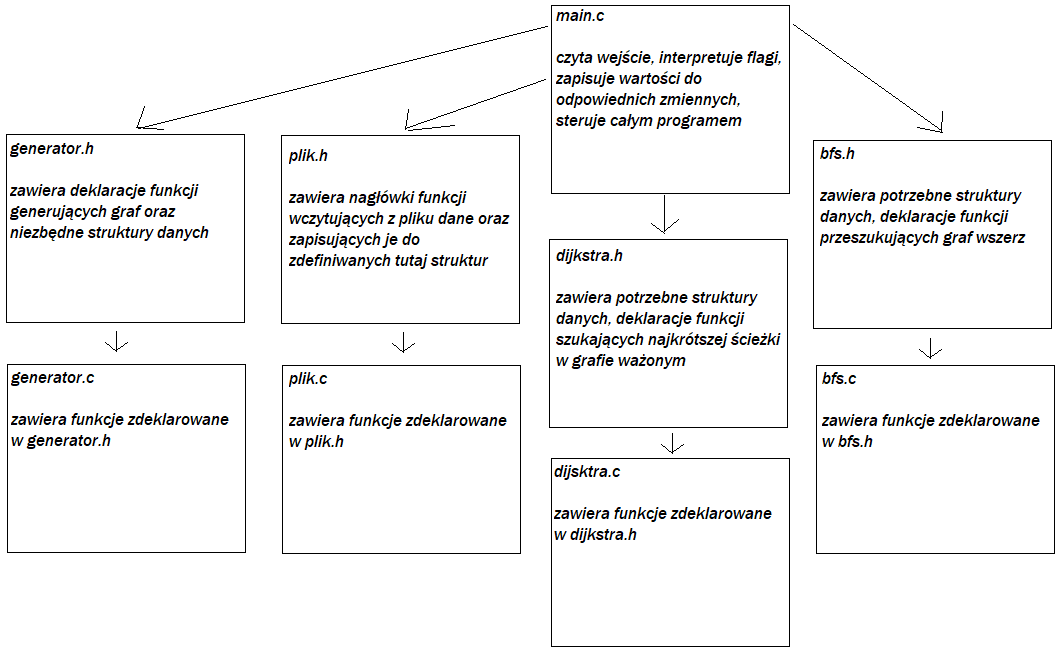
\includegraphics[width=0.9\textwidth]{moduly_programu2.png}
\caption{\label{fig:mod}Graficzna reprezentacja struktury programu (opracowanie własne)}
\end{figure}
\begin {itemize}
\item main.c zawiera:
    \begin {itemize}
    \item \texttt{\footnotesize int readArguments(int argc, char** argv)} - funkcję odpowiedzialną za rozpoznanie podanych argumentów, zwracającą 0 przy poprawnym działaniu i 1 przy błędnym działaniu.
    \item \texttt{\footnotesize int main(int argc, char**argv)} - funkcję zapewniającą obsługę wszystkich pozostałych funkcji.
    \item \texttt{\footnotesize typedef struct graph\_t} - strukturę, przechowującą graf
    \end {itemize}

\item plik.h zawiera funkcje:
    \begin{itemize}
        \item \texttt{\footnotesize int readFile(char* in)} - odpowiedzialną za czytanie danych wejściowych, zwracającą 0 przy poprawnym działaniu i 1 przy błędnym działaniu.
        \item \texttt{\footnotesize int writeFile(char* out)} - odpowiedzialną za wypisanie danych wejściowych, zwracającą 0 przy poprawnym działaniu i 1 przy błędnym działaniu
        \item \texttt{\footnotesize int writeResults(char* out)} - odpowiedzialną za wypisanie wyników, zwracającą 0 przy poprawnym działaniu i 1 przy błędnym działaniu
    \end{itemize}
\item generator.h zawiera funkcje:
    \begin{itemize}
        \item \texttt{\footnotesize int generateWeigh(double low, double high)} - odpowiedzialną za generowanie wag dla krawędzi w przedziale od low do high
        \item \texttt{\footnotesize int generateConnetions(int a)} - odpowiedzialną za generowanie krawędzi w zależności od wartości \texttt{\footnotesize a}, gdzie \texttt{\footnotesize a} oznacza tryb pracy generatora
    \end{itemize}
\item bfs.h zawiera funkcje:
\begin{itemize}
    \item \texttt{\footnotesize int bfs(graph\_t* graph)} - odpowiedzialną za przeszukiwanie grafu wszerz
\end{itemize}
\item dijkstra.h zawiera funkcje:
\begin{itemize}
    \item \texttt{\footnotesize int dijkstra(graph\_t* graph)} - odpowiedzialną za znajdowanie najkrótszej ścieżki w grafie
\end{itemize}
\end{itemize}



\section{Algorytm BFS}
Działanie algorytmu BFS, czyli algorytmu przeszukiwania grafu wszerz, można streścić następująco: \\ \\
Wybieramy wierzchołek startowy. Następnie odwiedzamy po kolei wszystkie wierzchołki sąsiadujące z wierzchołkiem startowym. Następnie odwiedzamy po kolei wszystkie nieodwiedzone wierzchołki sąsiadujące z wierzchołkami sąsiadującymi z wierzchołkiem startowym i tak dalej…\\
Niezbędna do funkcjonowania BFSa jest kolejka FIFO (odnośnik do pkt 2.) oraz tablica która dla każdego wierzchołka będzie posiadała informację o jego stanie: \\

0  – nieodwiedzony (kolor biały) \\
1 – dodany do kolejki lecz nieodwiedzony (kolor szary) \\
2  - odwiedzony (kolor czarny) \\

\textbf{Złożoność pamięciowa}
 \\Dla wykorzystanej w tym programie listy sąsiedztwa złożoność pamięciowa opisana jest wzorem O(V+E) gdzie: V - liczba wierzchołków, E - liczba krawędzi.\\

\textbf{Złożoność czasowa}
\\Pesymistyczny przypadek to taki, gdy algorytm musi odwiedzić wszystkie wierzchołki oraz krawędzie, wtedy złożoność czasowa wynosi O(V+E), gdzie V - liczba wierzchołków, E - liczba krawędzi.
\section{Algorytm Dijkstry}
Algorytm dijkstry służy do znajdowania  \textbf{najkrótszej ścieżki} w grafie ważonym. Przez \textbf{ścieżkę} pomiędzy dwoma wierzchołkami rozumiemy kolejno uporządkowane wierzchołki, które należy odwiedzić aby dostać się z wierzchołka startowego do końcowego. Z kolei \textbf{najkrótszą} ścieżką jest ta, której suma wag krawędzi jest najniższa. Algorytm Dijkstry, podczas działania, znajduje najkrótsze ścieżki do każdego wierzchołka do którego można dojść z wierzchołka startowego
\\ \\
Niezbędne do poprawnego działania będzie utworzenie:
\begin {itemize}

\item Tablicy d[V], gdzie V oznacza liczbę wszystkich wierchołków w grafie. Przechowywać będzie ona informację o długości aktualnej najkrótszej ścieżki z wierzchołka startowego do danego wierzchołka. Dla wierzchołka startowego s, d[s] przyjmuje początkowo wartość 0, a dla każdego innego nieskończoność.
\item Tablicy p[V], gdzie V oznacza liczbę wszystkich wierchołków w grafie. Przechowywać będzie ona informację o poprzednim wierzchołku w najkrótszej ścieżce do danego wierzchołka. Początkowo jest pusta.
\item Kolejki priorytetowej opartej na strukturze kopca. W kolejce tej początkowo będą wszystkie wierzchołki, a priorytetem wyciągania elementów z niej będzie najniższa wartość d[v] dla danego wierzchołka v.\\

\end{itemize}
Algorytm Dijkstry można przedstawić następująco: (źródło: pl.wikipedia.org)\\

\begin{figure}[t]
\centering
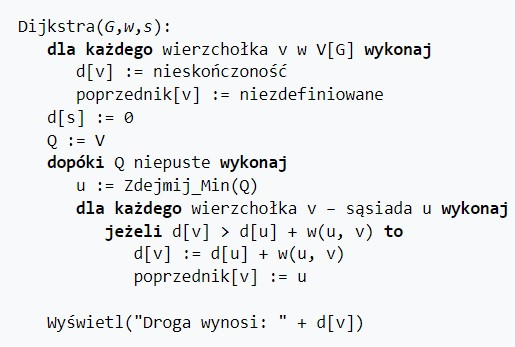
\includegraphics[width=0.9\textwidth]{alg_dijkstra.jpg}
\caption{\label{fig:dij}Algorytm Dijkstry (źródło: pl.wikipedia.org)}
\end{figure}




\section{Testowanie}
Poprawność działania programu należy sprawdzić kolejno testami, oraz wyniki porównać z wcześniej przygotowanymi danymi:
\begin{itemize}
    \item \texttt{void testAllRandModeGenerator(int rows, int cols, double minValue, double maxValue, int dec);} - funkcja sprawdzająca poprawność działania generator w trybie AllRandMode
    \item \texttt{void testRandWeightModeGenerator(int rows, int cols, double minValue, double maxValue, int dec);} - funkcja sprawdzająca poprawność działania generator w trybie RandWeightMode
    \item \texttt{void testConModeGenerator(int rows, int cols, double minValue, double maxValue, int dec);} - funkcja sprawdzająca poprawność działania generator w trybie ConMode
    
    
    \item \texttt{int testBFS(int start, int end);} - funkcja sprawdzająca poprawność działania algorytmu BFS
    \item \texttt{double testDijkstra(int start, int end);} - funkcja sprawdzająca poprawność działania algorytmu Dijkstry 

\end{itemize}

\section{Źródła}
\begin{enumerate}
    \item https://pl.wikipedia.org
\end{enumerate}


\end{document}
